%---------------------------------------------------------------------------------
\chapter{Introduction}
\label{chap:introduction}
%---------------------------------------------------------------------------------

%============================================== Background
\section{Background}
Recently, diffusion models \cite{nips_ddpm} \cite{iclr_ddim} \cite{lu2022dpm} have broken the leading performance of Generative Adversarial Networks (GANs) \cite{NIPS2014_5ca3e9b1} on image generation task and become the new state-of-the-art deep generative models. 
They have drawn great attention of AI researchers and have been rapidly applied to various generation tasks, such as image \cite{highresLDM}\cite{diff_autoencoder}, video\cite{videoDM}, audio\cite{oord2016wavenet}, natural language\cite{brown2020language} and multimodality \cite{url_stable} \cite{url_dalle2} \cite{cvpr_tcig}. 
Essentially, diffusion models consist of two processes: forward process and reverse process. In the forward process, a sample $x_0$ is perturbed into $x_T$ by progressively injecting Gaussian noise from time step $t=0$ to $t=T$, where $x_T$ becomes approximate pure noise and loses all structure of $x_0$. In the reverse process, starting from Gaussian noise $x_T$, diffusion models learn to denoise the data gradually until $t=0$, arriving at a new sample. Since the reverse process is to generate samples, it is also called sampling process. 
Unlike other generative counterparts such as GANs, variational autoencoders (VAE)\cite{kingma2013auto}, autoregressive models\cite{van2016conditional} and normalizing flows \cite{kingma2018glow} \cite{rezende2015variational} whose generation process is only one-time pass, diffusion models demand multiple iterative steps to generate sample.

Ideally, diffusion sampling process should be continuous and the step count $T\rightarrow\infty$. This would be convenient for mathematical modeling and analysis \cite{song2020score}.
But in practice sampling process is discretized and $T$ is assigned a reasonable value, such as $T=1000$ in paper \cite{nips_ddpm}. Such discretization will cause error because the discretized trajectory will deviate from the continuous one. Meanwhile, diffusion models themselves also have prediction error: the mismatch between predicted noise (or $x_0$) and the ground truth. And such prediction error will cause fitting error in sampling process.
As elaborated in paper \cite{zhang2022deis}, both of the discretization error and fitting error will thwart the sampling quality. That is illustrated in Fig \ref{fig:error-d-vs-p}.
% So there is dilemma when discretizing the sampling trajectory: more steps mean closer to ground truth trajectory, but slower in generation; and vice versa.

\begin{figure}[t] 
\centering
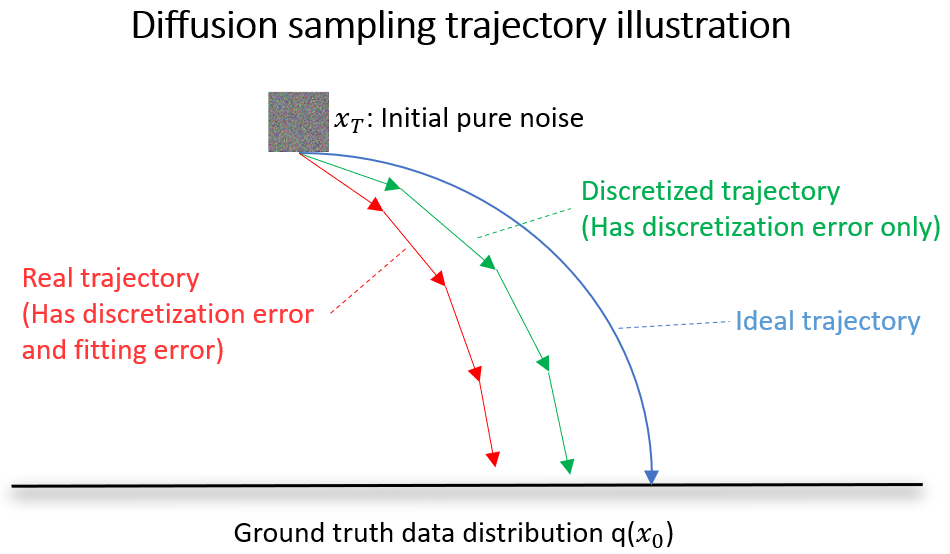
\includegraphics[width=0.45\textwidth]{figure/Error_discretization_vs_prediction.png}
\caption{Sampling trajectory illustration. In diffusion sampling process, there are two kinds of error: discretization error and fitting error. 
    The former happens when discretizing sampling process; and the latter is due to the mismatch between prediction and ground truth.}
\label{fig:error-d-vs-p}
\end{figure}

%============================================== Motivations
\section{Motivations}
Although new candidate technologies have been singled out for possible use in future aeronautical communications, the issue of spectral efficiency still continues to plague the aviation industry. Problems such as the coexistence of, and interference caused, by future and legacy communication systems on a crowded aeronautical spectrum are just a subset of potential issues which must be dealt with. Therefore, tackling the spectral crunch facing the aviation industry is a crucial but necessary step that must be taken in due time. Tackling the spectral efficiency issue will enable aeronautical communication links to better meet future data capacity demands while managing competition for spectral resources between current and future aeronautical communication technologies more efficiently. The urgency of improving spectral efficiency is also not unique to the aviation industry alone and is a challenging research problem in various other industries related to wireless communication systems \cite{dai2015non}. 

The study of spectral efficiency has always been a traditional problem in the communications literature. Related discussions, especially in recent years, have generally tackled the spectral efficiency problem from either a spectral utilization perspective or through employing advanced signal processing algorithms to exploit diversity advantages. Studies related to efficient spectrum utilization approaches have looked at various associated technologies such as Cognitive Radio (CR), enhanced modulation techniques and In-Band Full Duplex (IBFD) radio systems. Many others have also applied spectral efficiency techniques that have been studied in literature to a wide range of fields such as smart grids \cite{kouhdaragh2013cognitive}, wireless sensor networks \cite{he2014cr} and Long Term Evolution (LTE) networks \cite{zulhasnine2010efficient}. 

In terms of spectral efficiency for aeronautical communications, the application of LTE for A/G communications has been proposed in \cite{AlcatelSrat}. Concepts from the communications literature, such as adaptive modulations, have also been adopted for aeronautical usage in the form of AeroMACS \cite{budinger2011aeronautical}. However, the lack of available spectral resources is an underlying problem hampering further development of aeronautical communications technology. Therefore, more can be done in this aspect to further boost spectral efficiency for aeronautical communications.

%============================================== Objective of Work
\section{Objective of Work}
It is clear from the earlier discussions that the communication systems of both manned and unmanned aerial vehicles must utilize the limited aeronautical spectrum efficiently. One way to tackle the aeronautical spectrum crunch is to transmit more data per channel usage. Although an adaptive modulation-based ACS has been proposed in the form of AeroMACS \cite{budinger2011aeronautical}, modulation schemes that are suitable for aeronautical communications can also be studied to improve the data rate per channel usage, which is explored in the current work. To this end, the major milestones pertaining to suitable modulation schemes for aeronautical communications are summarized below.

%==============================================
\subsection{Major Milestones: Modulation Schemes}
\begin{itemize}
	\item The Quad State-Paired QPSK (QS-PQPSK), proposed in \cite{tan2016quad} to improve the data rate of current A/G links, was simulated for various aeronautical communications scenarios. In particular, the bit error rate (BER) of the QS-QPSK was compared against differential 8 phase shift keying (D8PSK) under  combinations of Rician and Rayleigh fading where it was found that the former outperforms the latter.
	\item To further improve the BER performance of QS-PQPSK, a Space Time Block Coded QS-PQPSK (STBC QS-PQPSK) was proposed. The BER of the proposed STBC QS-PQPSK was compared against 8PSK, QS-PQPSK and Rotative QPSK (RQPSK), i.e., bench marked against modulation schemes carrying three bits per symbol. In a Rayleigh flat fading channel, the proposed STBC QS-PQPSK outperforms 8PSK, QS-PQPSK and RQPSK across the simulated SNR ranges. 
	\item When simulated in the various aeronautical communications scenarios, the proposed STBC QS-PQPSK also exhibited superior BER performance when compared against QS-PQPSK and D8PSK.
\end{itemize}

Another alternative to tackle the aeronautical spectrum crunch directly is to transit from half-duplex (HD) based ACSs to hybrid-duplex (HBD) or even full-duplex (FD), i.e., IBFD, based ACSs. HBD-ACSs consist of HD and FD nodes concurrently operating on the same spectrum while FD ACSs requires all nodes to operate in FD mode. Therefore, both HBD-based and FD-based ACSs can provide up to twice the spectral efficiency when compared to existing /legacy HD-based ACSs.

As a step towards transitioning from HD-based ACSs to FD-based ACSs, HBD-based ACSs can be considered to minimize potential disruption to the aviation community. In particular, the current work evaluates the performance of an HBD-ACS from the outage and finite signal-to-noise-ratio (SNR) diversity-multiplexing tradeoff (DMT) perspective. The outage and finite SNR DMT analysis is used to identify suitable operating scenarios for which the HBD-ACS outperforms existing /legacy HD-based ACSs. The major milestones pertaining to HBD-ACS for aeronautical communications are summarized below.

%==============================================
\subsection{Major Milestones: HBD-ACS}
\begin{itemize}
	\item The present work proposes an innovative approach for deriving closed-form expressions for outage probability for a II detector and a two-stage SIC detector in a Rician faded environment.
	\item It is shown that the proposed HBD-ACS attains superior outage performance over existing HD-ACS at low SNRs. At high SNRs, however, the outage performance of the proposed HBD-ACS is eclipsed by HD-ACS as the former becomes interference-limited at asymptotic SNRs. Nonetheless, we show through numerical simulations that the HBD-ACS can meet typical Quality-of-Service (QoS) requirements, e.g., frame error rate $\leq 10^{-3}$, at high SNRs for a range of interference levels through II and SIC detectors. 
	\item Closed-form finite SNR diversity gain expressions are derived for the II and SIC detectors under Rician fading. The asymptotic behavior of the derived finite SNR diversity gains for HBD-ACS and HD-ACS are proven and shown to be consistent with interference-limited outage behaviors at asymptotic SNRs.
	\item The proposed HBD-ACS is shown to achieve better diversity gains than HD-ACS at high multiplexing gains. Finite SNR DMT analysis reveals that operating at higher multiplexing gain causes the Rician $K$ factor, corresponding to the SOI, to have more impact on HBD-ACS outage performance. Additionally, reducing residual SI and interference from AS-1 leads to steeper decay of outage probability, improving the finite SNR DMT curve of the proposed HBD-ACS as a consequence.
\end{itemize}
 
 %============================================== Report Outline
\section{Report Outline}

The remaining part of this report is organized as follows.

The state-of-the-art and suitable spectral efficiency techniques for aeronautical communications are discussed in Chapter II. In particular, future candidate technologies for various flight domains in aeronautical communications are presented as part of the state-of-the-art. Studies on aeronautical channel modeling are then presented, before further discussions on suitable spectral efficiency techniques for aeronautical communications 

In Chapter III, improvements to aeronautical waveforms over aeronautical communication channels are discussed. In particular, a new modulation scheme is proposed, simulated and compared, over various fading environments, against existing modulation schemes used in aeronautical communications.

Discussions on a proposed HBD system for aeronautical communications are presented in Chapter IV. The performance of the proposed HBD system is evaluated from both the outage probability and finite SNR DMT perspective, and is compared against existing HD systems.

Finally, future extensions of the works in Chapter III and Chapter IV are presented before the conclusion of this report in Chapter V.

%
%an overview of aeronautical communication links and systems in Chapter II. Discussions in Chapter II will span VHF-band (Very High Frequency-band), L-band and C-band systems for both A/G and A/A communication links. Channel access methods will also be briefly mentioned. We will then present suitable spectral efficiency techniques and its respective state-of-the-art that can be adopted for aeronautical communications in Section III. Finally, potential research topics will be deliberated in Section IV before the conclusion of this paper in Section V.
%
%This report is organized as follows:
%
%Chapter 2 provides ....................................
%
%Chapter 3 reviews ....................................
%
%Chapter 4 discusses ....................................
%
%In Chapter 5, we propose ....................................
%
%Finally, we conclude in Chapter 6, where we also discuss about the
%directions and schedule of our future research.
